\documentclass[a4paper,11pt]{article}
\usepackage{amsmath,amsthm,amssymb}
\usepackage[utf8]{inputenc}
\usepackage[english,russian]{babel}
\usepackage[export]{adjustbox}
\usepackage{graphicx}
\usepackage{pgfplots}
\usepackage{textcomp}

\graphicspath{{pictures/}}
\DeclareGraphicsExtensions{.pdf,.png,.jpg}
\leftskip=-0cm 
\rightskip=-0cm
\voffset = -3cm
\hoffset = -3cm
\textwidth = 550pt
\textheight = 770pt
\pgfplotsset{width=10cm,compat=1.9}


\begin{document}
\Large
HW7
\\
1

\begin{center}
\center{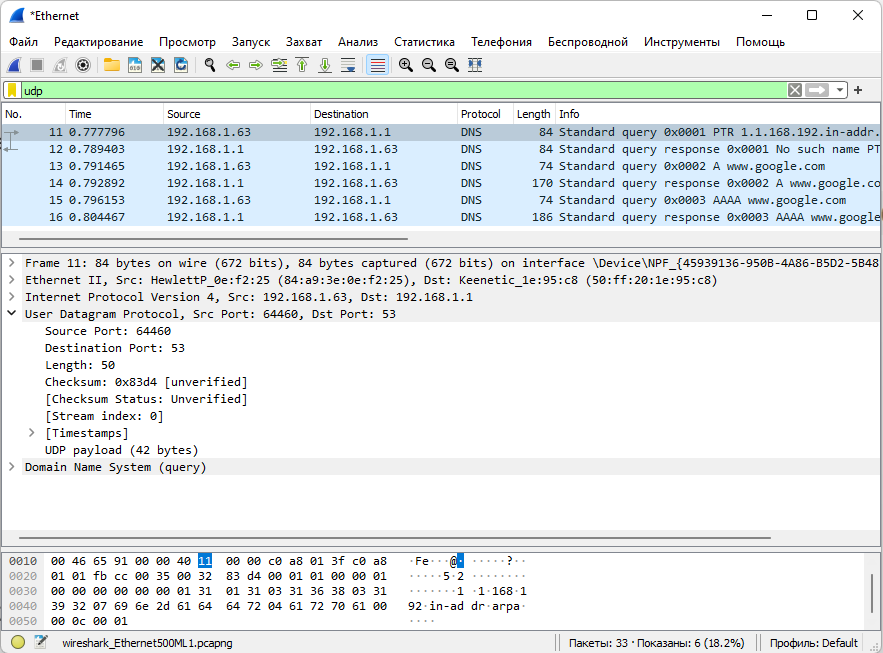
\includegraphics[width =\textwidth]{screenshots/1.png}}
\label{fig:image}
\end{center}
4 поля:\\
Source Port: 64460\\
Destination Port: 53\\
Length: 50\\
Checksum: 0x83d4 [unverified]

Длина каждого поля 2 байта

Length = 8 (заголовок) + 42 (данные)

Length - 16-битное число, значит не больше $2^{16} - 1 - 8 = 65527$ (так как заголовок тоже учитывается)

Port тоже 16-битное число, то есть до $2^{16} - 1$

\begin{center}
\center{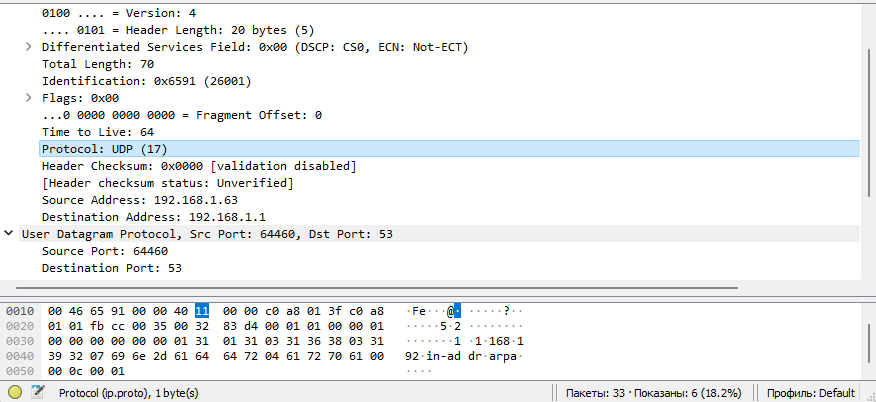
\includegraphics[width =\textwidth]{screenshots/2.png}}
\label{fig:image}
\end{center}
Номер протокола 17 в десятеричной или 11 в шестнадцатеричной

\begin{center}
\center{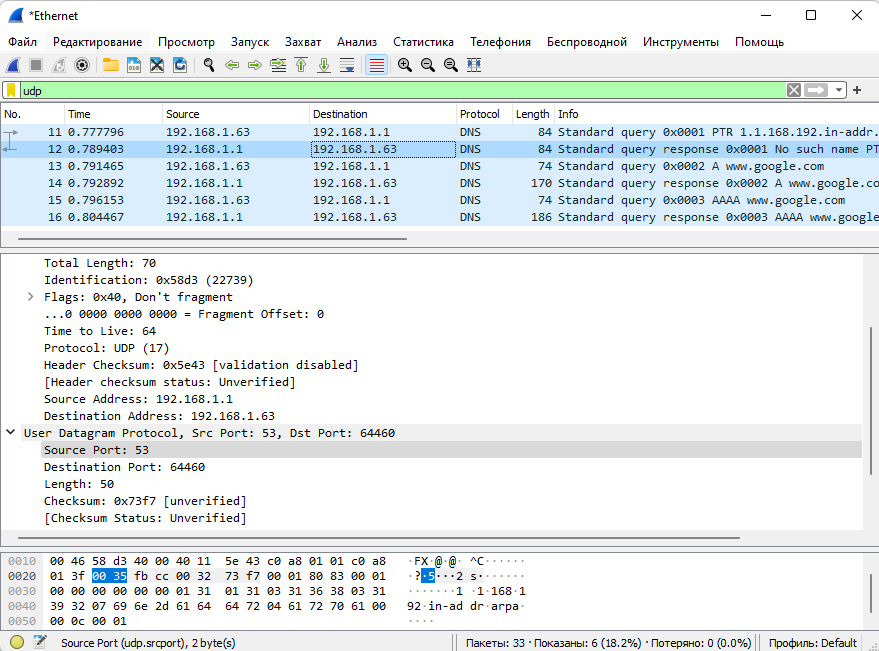
\includegraphics[width =\textwidth]{screenshots/3.png}}
\label{fig:image}
\end{center}
В ответном пакете \\
Source Port: 53\\
Destination Port: 64460

То есть порты поменялись местами
\end{document}








































